\chapter{Resultados}\label{chapter:results}

En este cap\'itulo que sigue presenta los hallazgos clave de nuestro análisis, enfocándose en los resultados relativos a la relación entre el periodo preferido y la excentricidad en diferentes áreas visuales, así como su relevancia en la lateralización hemisférica.

\section{Análisis de la elación entre el Tamaño de los pRF y la Excentricidad}

\begin{figure}[h]
	\centering
	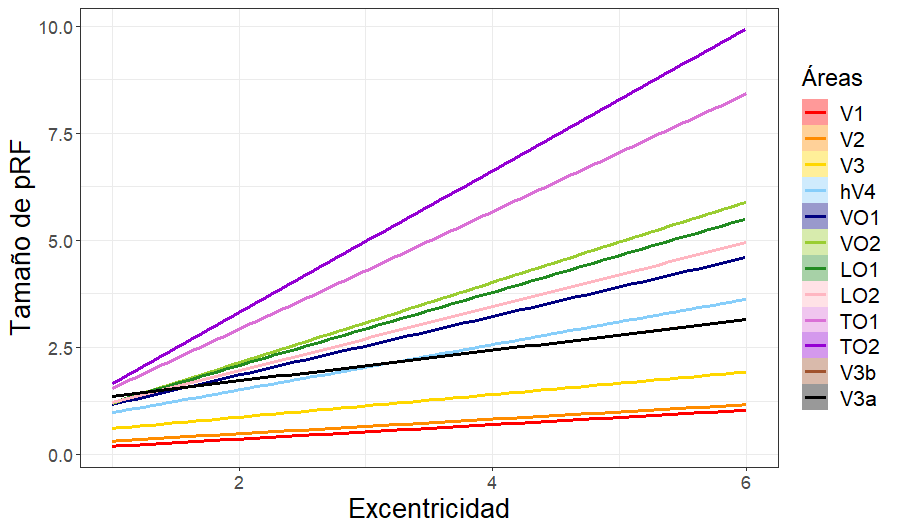
\includegraphics[scale=0.6]{Graphics/size_vs_eccen_bayesian}
	\caption{Gráfico que representa la relación entre el tama\~no de pRF y la excentricidad en las diferentes áreas visuales analizadas.}
	\label{fig:sigma_vs_eccen}
\end{figure}

Aunque no constituye el enfoque principal de este estudio, se llevó a cabo un análisis adicional para examinar la relación entre el tamaño del pRF y la excentricidad en el campo visual. En la Figura \ref{fig:sigma_vs_eccen}, presentamos las rectas de regresión correspondientes a estas variables. Observamos que el tamaño del pRF tiende a incrementarse con la excentricidad en el campo visual, una tendencia que se manifiesta consistentemente a través de las diferentes áreas examinadas. De manera notable, la pendiente de estas rectas de regresión muestra un aumento progresivo al pasar de áreas visuales tempranas, como V1-V3, a áreas de procesamiento visual de nivel superior, tal como TO1. Este hallazgo está en consonancia con investigaciones previas y refuerza la comprensión de que el tamaño del pRF se expande con la complejidad funcional y jerárquica de las áreas visuales \todo{añadir referencias pertinentes}.

\section{Análisis de la Relación entre el Período Preferido y la Excentricidad}

En la figura \ref{fig:pp_vs_eccen}, se puede observar que en la mayoría de las áreas visuales analizadas, se cumplen los supuestos de que el período preferido tiende a aumentar con la excentricidad. Sin embargo, es importante destacar que existen variaciones en este patrón.

En áreas visuales como hV4 y VO1, se observa una pendiente de crecimiento negativa. Este hallazgo sugiere que, a medida que la excentricidad aumenta, el período preferido tiende a disminuir en lugar de aumentar. Este comportamiento atípico resalta la diversidad de respuestas visuales en diferentes regiones corticales.

Además, en áreas visuales superiores como LO1, LO2, TO1 y TO2,  se evidencia un aumento del pendiente del período preferido con respecto a la excentricidad, comparado con las áreas visuales tempranas. Esta observación indica que estas áreas específicas muestran un patrón consistente de incremento en el período preferido a medida que nos alejamos del punto central de la visión.

Este análisis proporciona una comprensión más completa de cómo la excentricidad puede modular el período preferido en diversas áreas visuales, destacando la necesidad de considerar la heterogeneidad funcional en la corteza visual.

\begin{figure}
	\centering
	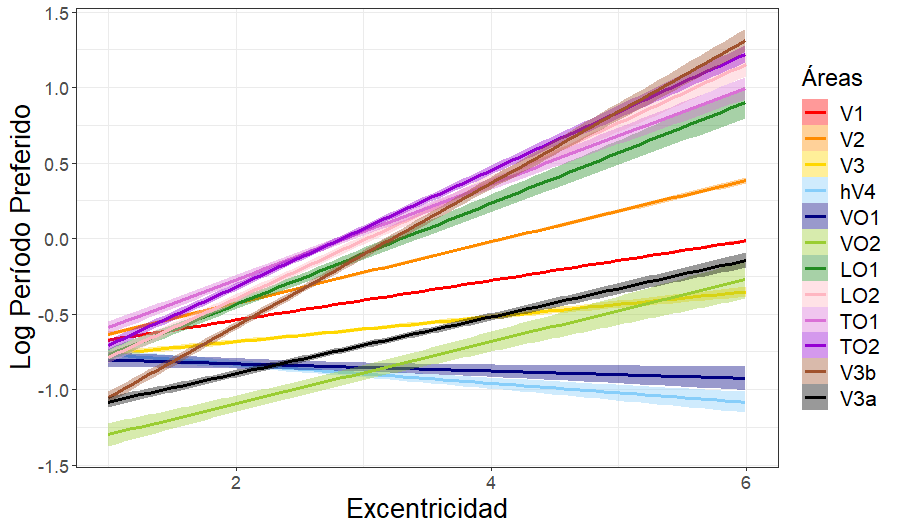
\includegraphics[scale=0.6]{Graphics/pp_vs_eccen}
	\caption{Gráfico que representa la relación entre el logar\'itm del per\'iodo preferido de los v\'oxeles y la excentricidad, en las 12 áreas visuales analizadas.}
	\label{fig:pp_vs_eccen}
\end{figure}

\section{Resultados del Modelo Lineal Mixto para Frecuencias Espaciales en función de Excentricidad y Hemisferio}

\begin{figure}
	\centering
	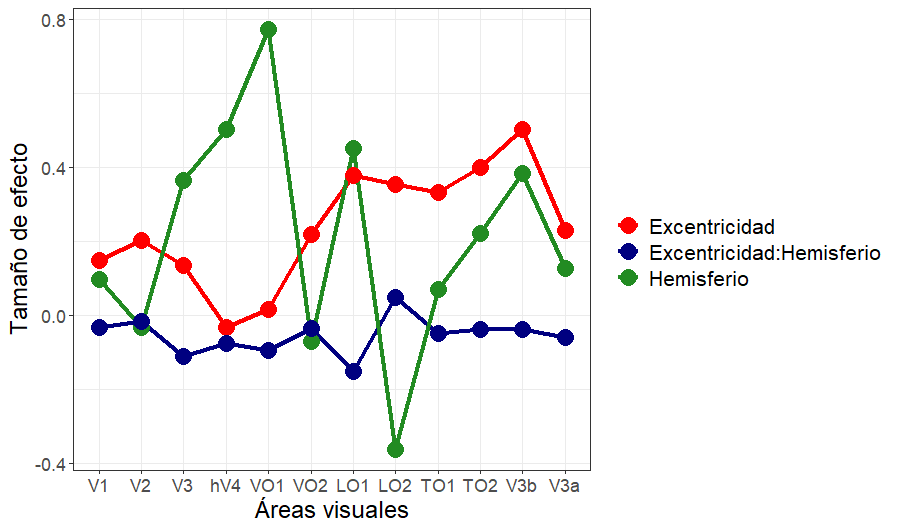
\includegraphics[scale=0.6]{Graphics/effect_size_coef_pp}
	\caption{Representación gráfica de los coeficientes estimados para las variables fijas del modelo lineal mixto \ref{mlm_pp}.}
	\label{fig:coeff}
\end{figure}

\begin{figure}
	\centering
	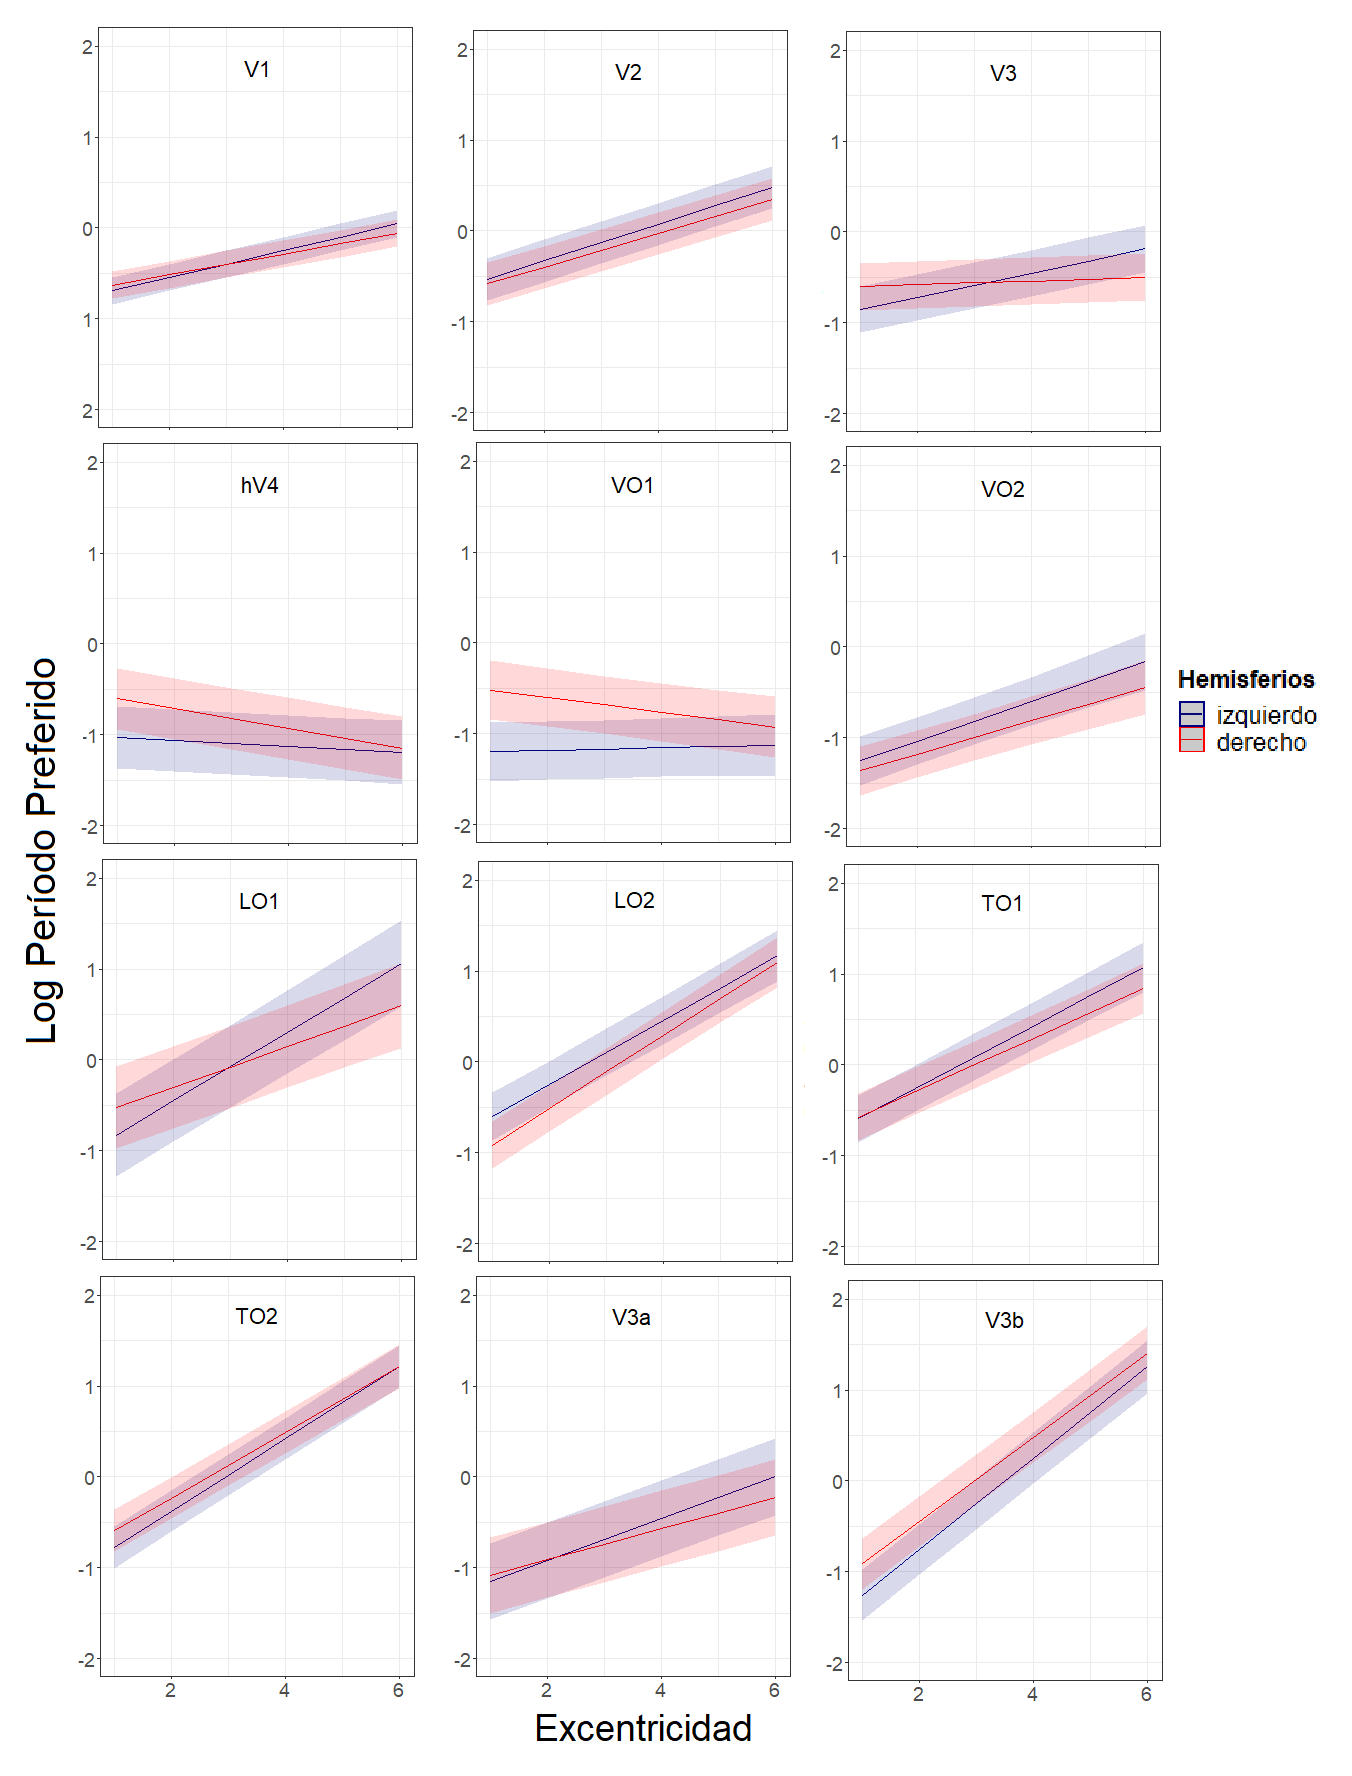
\includegraphics[scale=0.6]{Graphics/compuesto_rois_pp_vs_eccen_hem}
	\caption{Conjunto de gráficas representando la relación entre el logaritmo del per\'iodo preferido de los v\'oxeles y la excentricidad en los dos hemisferios cerebrales, para las 12 áreas visuales analizadas.}
	\label{fig:hem}
\end{figure}

A continuación, se aborda el núcleo central de esta tesis: el análisis del impacto del hemisferio cerebral sobre el per\'iodo preferido. Los resultados obtenidos del modelo lineal mixto, aplicado a las frecuencias espaciales de estímulos visuales, se detallan en la Figura \ref{fig:mlm_results_pp}. En esta figura, las filas ilustran las diferentes áreas visuales analizadas mediante el modelo \ref{mlm_pp}, mientras que las columnas representan las variables fijas del modelo con sus respectivos resultados estimación de los coeficientes (Coef), error estándar (SE), t-valor (t-val) y el factor de Bayes de la comparaci\'on de cada uno de los modelos propuestos en la secci\'on \ref{mlm}.

En el modelo \ref{mlm_pp} la variable de interés es "periodo preferido", que es el inverso de la frecuencia espacial. Se modela su relación con la excentricidad y el hemisferio. Además, se incluyeron efectos aleatorios para los sujetos y los estímulos. 

En la figura \ref{fig:mlm_results_pp} se observa que salvo en V01 y hV4, el efecto de excentricidad es positivo (crece periodo con excentricidad) y significativo en la t de Student y por el factor de Bayes.  También crece la magnitud el efecto al pasar de áreas tempranas a arreas de orden superior (confirmando lo visto en la figura XX.  En hV4 el coeficiente es negativo, aunque de menor tamaño que para otras areas, y significativo por la t de Student y el factor de Bayes. VO1 el coeficiente es muy pequeño, y no significativo.

Es llamativo que hay un efecto de hemisferio significativo en casi todas las áreas con excepción de V02, pero con coeficientes pequeños en V1, V2, TO1, y V3A. En las demás áreas (V3, hV4, VO1, LO1, LO2, TO2, V3B) el periodo es significativamente mayor en hemisferio derecho que el izquierdo, y mayor en V01, hV4 y LO1 (ver fFgura ***). Las interacciones entre excentricidad y hemisferio, aunque en muchas áreas fueron significativas, resultaron de poca magnitud en todas las áreas examinadas salvo V3 y LO1.




\begin{figure}
	\centering
	
\includegraphics[scale=0.8]{Graphics/table_pp}
	\caption{Tabla que resume los resultados del modelo lineal mixto empleado para analizar el logaritmo del periodo preferido de los voxeles en diferentes áreas visuales. Cada fila representa los resultados del modelo para una área visual específica. Para cada variable fija del modelo, la tabla muestra la estimación del coeficiente (Coef), el error estándar (SE) y el valor t (t-val). Además, se incluye el factor de Bayes (BF10) para la comparación entre modelos: el BF10 en la columna 'Excentricidad' corresponde a la comparación entre el modelo \ref{m_1} y \ref{m_2}; en la columna 'Hemisferio', se refiere a la comparación entre el modelo \ref{m_2} y \ref{m_3}; y en la columna 'Excentricidad:Hemisferio', a la comparación entre los modelos \ref{m_3} y \ref{mlm_pp}.}
	\label{fig:mlm_results_pp}
\end{figure}






